\chapter{Propagating the Uncertainty of Stereo Images}
This chapter details the work conducted on the propagation of uncertainty from images into the cost curves of dense matching problems. We consider a simple model of uncertainty on the input images, a dependency model between the uncertain intensities of the images, and estimate the resulting uncertainty on the output cost curves. This chapter takes up work and data already published \cite{malinowski_copulas_2022, malinowski_uncertainty_2023, malinowski_robust_2024}.

\section{Sources of uncertainty in stereo matching}
\comroman{Points à aborder: Atmospheric correction, vibration, resolution of a pixel, discretization.
CO3D mission will not have the epipolar line correction problem that is encountered with pleiades images.
Epipolar line rectification for Pléiades is a problem that is not dealt here.}

To maintain simplicity in this section, we will not consider panchromatic images, such as Pléiades products, encoding the reflectance values as positive integer, usually contained in $[0, 5000]$. Instead, we consider grayscale images that have intensity levels quantified within the range $[0, 255]$, which will represent our measurable space $\X$. We hypothesize that a pixel's intensity value can deviate by no more than $1$ level from its observed value, with the observed value being the most likely. This hypothesis arises from the noise of the sensor capturing the image, from pre-processing steps (see section \ref{sec:classical_stero_pipeline}) or from the quantification of observed radiometric values into integers. We assume this simple hypothesis to keep our explanation straightforward. Consequently, we model the uncertainty of each pixel $p\in I_L,I_R$ intensity with a possibility distribution $\pi$, centered around the observed intensity $i_p\in[0,255]$:
\begin{equation}
    \pi(i_p)=1,\quad \pi(i_p\pm1)=\alpha\,,
\end{equation}\label{eq:pixel_possibility}
with $\alpha \in [0,1]$. The $\pm$ indicates that both positive and negative values are considered. In our simulation, $\alpha = 0.3$ for pixels in the left image and $\alpha = 0.4$ for pixels in the right image. We use different values of $\alpha$ for the left and right images because the uncertainty model may vary between images due to differences in exposure, noise levels, or camera calibration. This model effectively states that we accept any probability distribution supported within $[i_p - 1, i_p + 1]$ where the probability measure $P$ satisfies $\{P(A) \leq \sup_{i \in A} \pi(i)\}$ as an acceptable model for our uncertainty. The mass distribution function $m_p$ associated to this credal set possesses two focal sets $a^p$:
\begin{eqnarray}
    &m_p(a^p_1=\opi i_p, i_p\cli)=1-\alpha\,\nonumber\\
    &m_p(a^p_2=\opi i_p-1, i_p + 1\cli)=\alpha\,\label{eq:pixel_mass}
\end{eqnarray}
with $\opi\cdot, \cdot\cli$ referring to integer intervals. In particular, $\opi i_p, i_p\cli$ correspond to the singleton $\{i_p\}$.

It is important to note that in this disparity estimation problem, we only account for the uncertainty in our input image intensities, without considering the uncertainty in our cost function's ability to correctly identify the true disparity as its minimum. In other words, we do not account for the uncertainty arising from the difference between ``two patches are very similar'' and ``the pixels at the center of the patches are homologous''. To better illustrate this, imagine a scenario where two pixels should be matched, but the surrounding patches are dissimilar. In this case, the cost function between those two patches would be high, potentially leading to the selection of a different patch with a lower cost function as the estimated disparity. The correct disparity would not be the minimum of the cost curve.

We consider the Sum of Absolute Differences (SAD) as our cost function, defined as follows. Given patches $W_L\subset I_L$ and $W_R\subset I_R$ of the same shape with $n$ pixels (usually squares):
\begin{align}
    \mathrm{SAD}(W_L, W_R) = \sum_{(p_i, q_i)\in (W_L, W_R)}|I_L(p_i) - I_R(q_i)|\label{eq:SAD}
\end{align}
where $p_i$ and $q_i$ are pixels at the same position $i$ in their patch. For convenience purposes, we will refer to the Absolute Difference as AD. This cost function is not ideal compared to more complex state-of-the-art cost function (\cite{zbontar_stereo_2016}, \cite{laga_survey_2022}), but it is preferred here to focus on simplicity and to ease didactic explanations regarding uncertainty propagation. An illustration of the SAD cost function can be found in Figure \ref{fig:SAD}. An ideal cost function would generate a cost curve with a unique minimum corresponding to the correct disparity. In practice, such a function is hard to determine. There is no guarantee that the minimum is unique, nor that it corresponds to the correct disparity. 

\begin{figure}
    \centering
    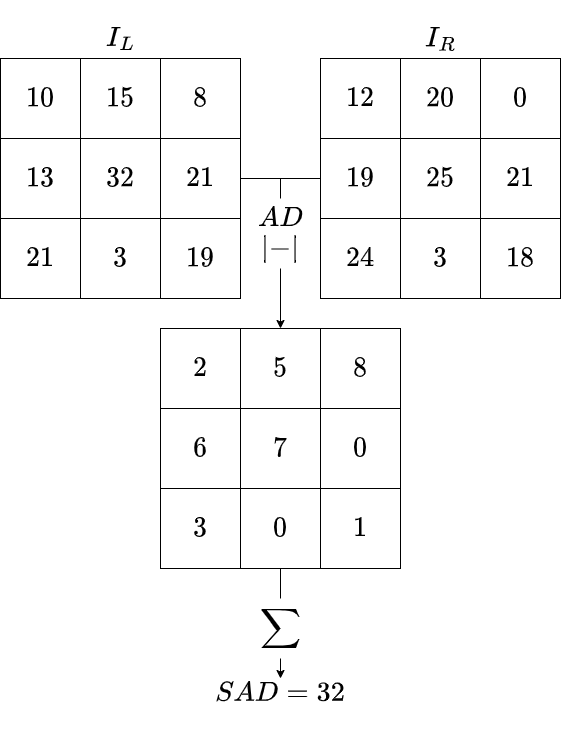
\includegraphics[width=0.5\linewidth]{Images/SAD.png}
    \caption{Diagram representing the $SAD$ cost function between two $3\times3$ patches.}
    \label{fig:SAD}
\end{figure}

\section{Propagation of the Uncertainty with Belief Functions}
This section will present how we can compute a Belief function on the matching cost curve values from the original beliefs as well as a copula representing the dependency between variables. We first detail how it can be done in the precise case, as the imprecise setting is similar. We use the case of the SAD cost function to illustrate the process.

First, let us present the propagation of uncertainty in the precise bivariate case. Let $f:\X_1\times\X_2\rightarrow\mathcal{Z}$ be a mapping and we define the random variables $Z$ as $Z=f(X,Y)$. 
When considering precise probabilities, the mass distribution $p_Z$ on atoms of $Z$ is:
\begin{align}
    \forall z\in\mathcal{Z}, p_Z(z)=\sum_{\substack{x_1,x_2\\z=f(x_1,x_2)}}p(x_1,x_2).
\end{align}

Determining every $(x,y)$, whose image by $f$ equals $z$, is not always trivial. This becomes even more complex when we are considering copulas with $n>2$ variables. Note that the joint probability $p(x_1,x_2)$ is computed using a H-volume, which is the sum of $2^n$ terms, also increasing exponentially with the dimension. In the continuous case, the H-volume is replaced with the density $h$ of the joint CDF. The density of $Z$ is thus:
\begin{align}
    p_Z(z) = \int_{\X_1}\int_{\X_2}h(x_1,x_2)\mathds{1}(f(x_1,x_2)=z)dx_1dx_2,
\end{align}
Here, $\mathds{1}$ refers to the characteristic function.

Similarly, belief functions can be propagated by replacing the mass on atoms with the mass associated to the joint belief function. Given the joint mass distribution function $m_\times$ constructed with a copula as in equation \ref{eq:joint_mass}, it is possible to compute the mass distribution function $m_Z$ of a random set $Z$ from $n$ marginal random sets:
\begin{align}
    \forall a^Z\subseteq\mathcal{Z}, m_Z(a^Z) = \sum_{\substack{a^1_i, \dots, a^n_j\\a^Z=f(a^n_1,\dots, a^n_j)}}m_\times(a^1_i, \dots, a^n_j)\label{eq:mass_propagated}
\end{align}
Computing the image of $f$ for every pair of focal sets $(a^1_i, \dots, a^n_j)$ is even more difficult than in the precise case, as we are computing reverse images of sets instead of real numbers. To illustrate how to propagate the uncertainty using belief functions and a copula, we will use the SAD cost function as an example.

The SAD is used to compute the similarity between $3\times3$ windows $W_L, W_R$. We use the mass distribution $m_p$ of Equation \eqref{eq:pixel_mass} to represent the uncertainty of each pixel $p$. For every pair of pixels $p\in I_L, q\in I_R$, we note $\mathrm{AD}_{pq}=|i_p - i_q|$. There exists $3$ focal sets related to the absolute difference:
\begin{itemize}
    \item $a^{\mathrm{AD}}_1$ is the image of the AD of $a^p_1$ and $a^q_1$
    \item $a^{\mathrm{AD}}_2$ is the image of the AD of $a^p_2$ and $a^q_1$ or $a^p_1$ and $a^q_2$
    \item  $a^{\mathrm{AD}}_3$ is the image of the AD of $a^p_2$ and $a^q_2$
\end{itemize}
The non-monotonicity of the absolute value around $0$ needs to be taken into account to compute their exact image through the AD:
\begin{align*}
    a^{\mathrm{AD}}_1&=\opi\mathrm{AD}_{pq},~\mathrm{AD}_{pq}\cli\,,\\
    a^{\mathrm{AD}}_2&=\opi\mathrm{AD}_{pq} - 1,~\mathrm{AD}_{pq} + 1\cli\text{ if }\mathrm{AD}_{pq}>0\,,\\
            &=\opi\mathrm{AD}_{pq},~\mathrm{AD}_{pq} + 1\cli\text{ otherwise }\,,\\
    a^{\mathrm{AD}}_3&=\opi\mathrm{AD}_{pq} - 2,~\mathrm{AD}_{pq} + 2\cli\text{ if }\mathrm{AD}_{pq}>1\,,\\
            &=\opi\mathrm{AD}_{pq} - 1,~\mathrm{AD}_{pq} + 2\cli\text{ if }\mathrm{AD}_{pq}=1\,,\\
            &=\opi\mathrm{AD}_{pq},~\mathrm{AD}_{pq} + 2\cli\text{ otherwise}\,.
\end{align*}

Bounds of the AD are then summed to obtain the final values of the SAD focal sets. The mass $m_{\mathrm{SAD}}$ of those focal sets are computed using equations \ref{eq:joint_mass} and \ref{eq:mass_propagated}. To represent the dependency between pixels of both windows, a Gaussian $18$-copula is used. Splitting the problem using lower dimension copulas is tempting, similarly to what can be done with vine copulas (\cite{czado_vine_2022}). However this is a complex problem that will not be explored in this thesis. We will instead work with Gaussian copulas, introducing a simple method for creating a correlation matrix. This will also allow us to present simple optimisation to reduce computation complexity and splitting the copulas into mutually independent groups of variables. 

\section{Leveraging specificities to accelerate computations}
\comroman{H Volume etc for SAD example, see IJAR.}

Determining the bounds of the SAD focal sets is mostly straightforward. However, computing the joint mass over two $3 \times 3$ windows is significantly more complex. For each combination of marginal focal sets, the mass $m_{\mathrm{SAD}}$ is computed using the $H$-volume of an $18$-copula, involving a sum of $2^{18}$ terms. Given that the uncertainty for each pixel is represented by $2$ focal sets, we need to evaluate $2^{18}$ combinations of these focal sets in total. This computation can thus become quite costly in memory and computation time, especially when computing it over a whole image. A strategy to reduce computation time is to leverage the fact that the focal sets derived from a possibility distribution (or equivalently from its necessity measure) form a nested family of sets. In the general case, propagating two necessity measures $\mathrm{Nec}_1:2^{\X_1} \rightarrow [0,1]$ and $\mathrm{Nec}_2: 2^{\X_2} \rightarrow [0,1]$ through a mapping $f: \X_1 \times \X_2 \rightarrow \mathcal{Z}$ using a copula $C$ does not result in a necessity measure, but rather a belief function.

For the special case where:
\begin{itemize}
    \item $\mathrm{Nec}_1$ and $\mathrm{Nec}_2$ are defined by symmetric uni-modal possibility distributions (typically triangular possibilities), and
    \item $f$ is a monotone function applied to a linear combination $\alpha X_1 + \beta X_2 + \gamma$, with $(\alpha, \beta, \gamma) \in \mathbb{R}^3$,
\end{itemize}
the focal sets of $Z = f(X_1, X_2)$ form a nested family of sets, which is a characteristic of necessity measures \cite{shafer_mathematical_1976}.

Indeed, the focal sets of $\mathrm{Nec}_{\X_1}$ and $\mathrm{Nec}_{\X_2}$ are families of nested sets that can be represented as:
\begin{align*}
    a_{ij} = \left[ \alpha \overline{X_1} + \beta \overline{X_2} + \gamma - (|\alpha| \Delta x^1_i + |\beta| \Delta x^2_j), \right. \\
                 \left. \alpha \overline{X_1} + \beta \overline{X_2} + \gamma + (|\alpha| \Delta x^1_i + |\beta| \Delta x^2_j) \right],
\end{align*}
where:
\begin{itemize}
    \item \( \overline{X_1} \) and \( \overline{X_2} \) denote the expected values of \( X_1 \) and \( X_2 \),
    \item \( \Delta x^1_i \) and \( \Delta x^2_j \) represent the variations or uncertainties associated with \( X_1 \) and \( X_2 \), respectively.
\end{itemize}

These sets form a nested family. When a monotone function is applied to these focal sets, the nesting property is maintained, although the symmetry of the sets might be lost. This implies that \(\mathrm{Bel}_Z\) (the belief function derived from \( Z \)) behaves as a necessity measure under these conditions.

On the other hand, for more sophisticated functions, such as multiplication, exponential functions, or sigmoid functions, the nesting property might not hold. It's often easy to find counterexamples where the nested nature of the focal sets is disrupted when such functions are applied. The upcoming example illustrates this situation.

\pagebreak